\chapterpage{Implementation and Development}
\mychapter{Implementation and Development}

This chapter documents how the design described in~\cref{chap:methodology} was translated into a working system. It covers the programming languages and third party technologies used, a detailed breakdown of the implementation across the interface, orchestration, storage, and algorithmic layers of the system, the testing and debugging strategy applied during development, and the version control and configuration management practices that governed the project's evolution.

\section{Programming Languages and Technologies Used}

The system is implemented entirely in \textit{Python 3.12.8}, chosen for its mature computer vision and deep learning ecosystem, rapid iteration speed, and first class support for the numerical and array processing libraries the pipeline depends on. Table~\ref{tab:techstack} summarises the technology stack used in the proposed system and the role of each component within the overall pipeline.

\begin{longtable}{|>{\raggedright\arraybackslash}p{2.8cm}|>{\raggedright\arraybackslash}p{2.4cm}|>{\raggedright\arraybackslash}p{8.9cm}|}
\caption{Technology stack and role of each component}
\label{tab:techstack}\\
\hline
\textbf{Technology} & \textbf{Category} & \textbf{Role in the System} \\
\hline
\endfirsthead

\hline
\textbf{Technology} & \textbf{Category} & \textbf{Role in the System} \\
\hline
\endhead

\textit{Python 3.12.8} & Language & Primary implementation language for the entire pipeline \\
\hline
OpenCV (\texttt{opencv-}\allowbreak\texttt{python}) &
Computer Vision &
Image/video I/O, CLAHE, Gaussian blur, Canny edge detection,
Haar-cascade detection, NMS, drawing/annotation \\
\hline
PyTorch \& (\texttt{torchvision}) & Deep Learning & Tensor operations and inference engine for the Four-Column MDNN density-regression network \\
\hline
Ultralytics (\texttt{ultralytics}) & Deep Learning & YOLOv8-nano person/head detector (sparse branch) \\
\hline
NumPy & Numerical Computing & Array manipulation for density maps, bounding boxes, and image tensors \\
\hline
SciPy & Scientific Computing & \texttt{scipy.\allowbreak optimize.\allowbreak linear\_\allowbreak sum\_\allowbreak assignment} (Hungarian algorithm) for multi-object tracking \\
\hline
Matplotlib & Visualization & Diagnostic plotting of density maps and count trends \\
\hline
% Polars & Data Processing & Lightweight tabular aggregation of per-frame statistics for video runs \\
% \hline
% Python \texttt{logging} & Diagnostics & Centralized, rotating-per-run logging and step-level latency profiling (\texttt{logger.py}) \\
% \hline
% \texttt{dataclasses} (stdlib) & Configuration Management & Type-safe, centralized hyper-parameter definitions (\texttt{config.py}) \\
% \hline

\end{longtable}

The choice of PyTorch and Ultralytics reflects the two deep learning components in the hybrid architecture: a general purpose pretrained object detector (YOLOv8) for the sparse branch, and a custom trained etwork for the dense branch. OpenCV was selected as the common substrate for all classical image processing operations (colour space conversion, filtering, edge detection, drawing) because it offers a single, well optimized, C++ backed API accessible from Python with negligible overhead, which matters given the system's per-frame latency budget.

\section{System Implementation}

It describes how the proposed passenger counting framework is realised as an operational software system. The implementation is divided into three major components: the user interaction layer, the backend processing layer, and the data management layer. These components collectively support input handling, passenger estimation, result generation, monitoring, and storage of system outputs.

\subsection{User Interaction Layer}

The system provides a lightweight user interaction mechanism through which an operator can process either image or video inputs. The operator first selects the required input type and then provides the corresponding media source. Basic input validation is performed before processing begins to ensure that the selected input can be processed successfully.

The command line interface used for input selection and system execution is illustrated in Figure~\ref{fig:cli-interface}. The interface provides a simple mechanism for selecting the input type and specifying the media source to be processed.

\begin{figure}[ht]
    \centering
    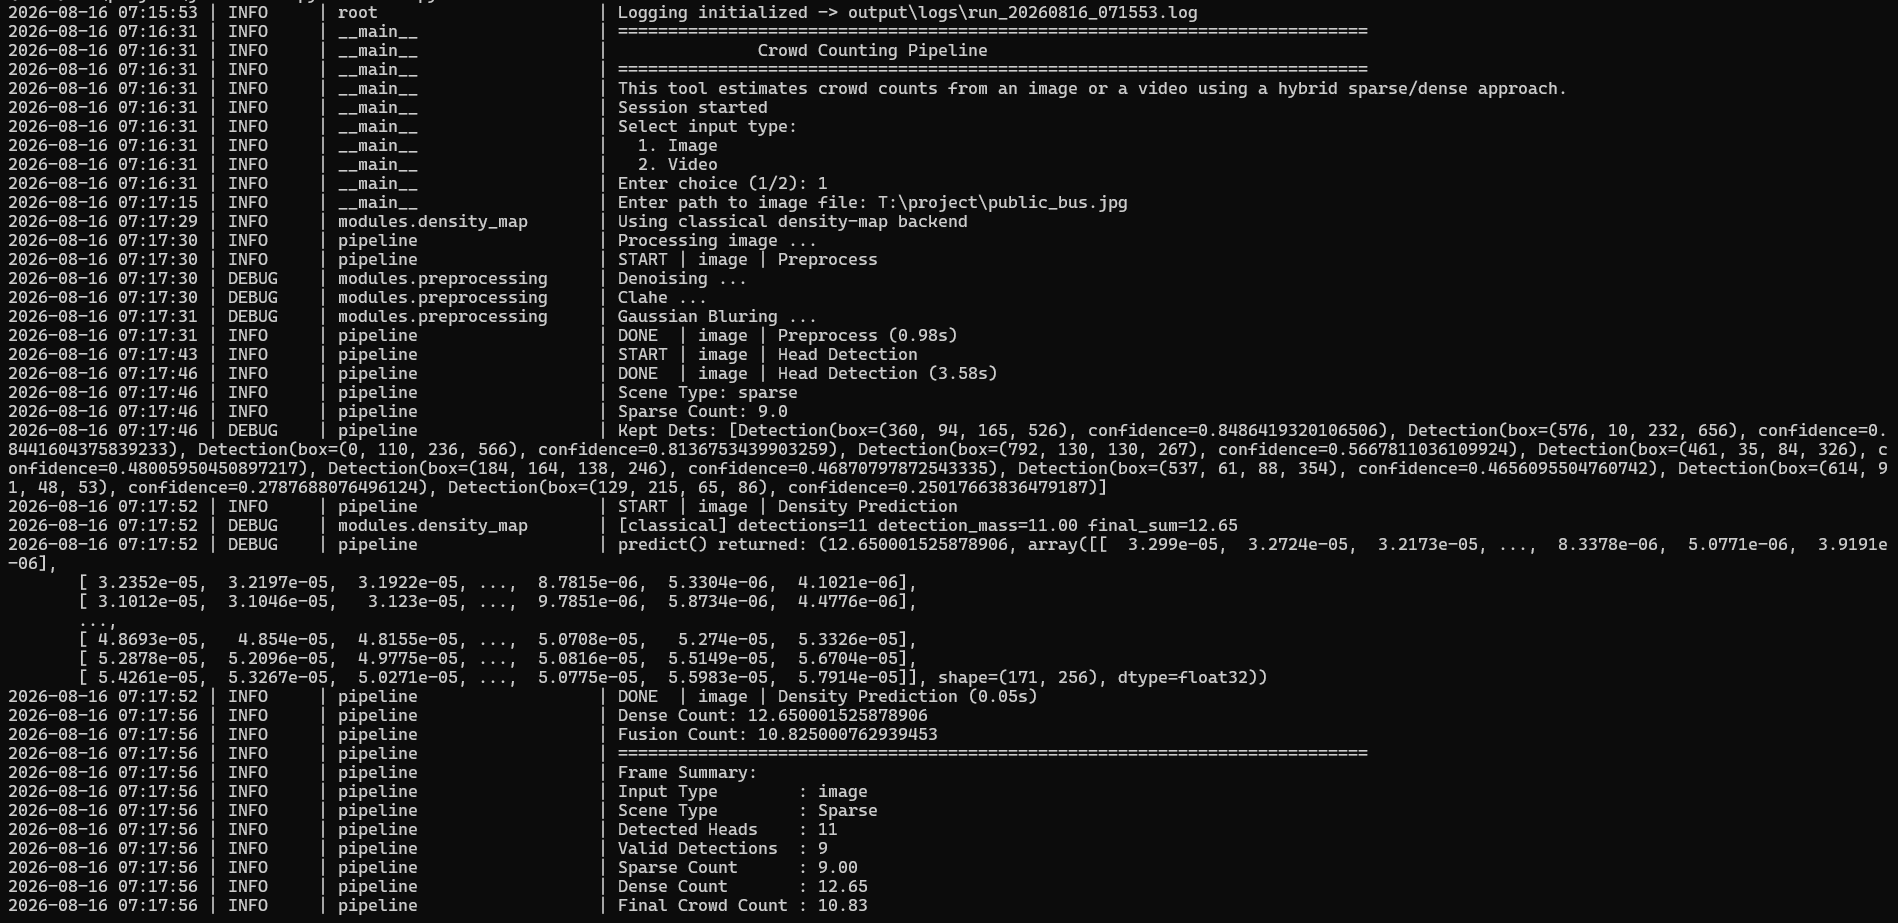
\includegraphics[width=1.00\textwidth]{figures/cli_interface.png}
    \caption{Command Line Interface for input selection and system execution}
    \label{fig:cli-interface}
\end{figure}

The interface is intentionally designed to minimise operational complexity while providing sufficient feedback to the user. During execution, the system reports processing progress, warnings, and relevant results. This allows the operator to monitor the analysis and identify potential problems during execution.

The system also provides visual representations of the generated results. Detected passengers or heads are displayed using bounding boxes, while the estimated crowd density information can be represented using heat map visualisations. The estimated passenger count and scene classification are displayed directly on the processed media, enabling the operator to visually inspect and validate the system output.

For video inputs, the processed frames are sequentially combined to produce an annotated output video. This provides a convenient representation of the counting process and allows the operator to review passenger detection and occupancy estimation results across the complete video sequence.

\subsection{Backend Processing Layer}

The backend constitutes the core processing layer of the system and is responsible for coordinating the different stages of the passenger counting workflow. It manages the flow of input data through preprocessing, passenger detection, density estimation, scene analysis, fusion, and result generation.

The processing architecture follows a modular and configuration driven approach. Parameters associated with image preprocessing, passenger detection, density estimation, tracking, and result fusion are maintained separately from the main processing logic. This separation allows the behaviour of individual components to be adjusted without requiring substantial modifications to the overall processing workflow. It also facilitates controlled experimentation with different parameter configurations.

The backend incorporates execution monitoring to support system reliability and performance evaluation. Individual processing stages are monitored to determine their execution time, allowing computationally intensive stages and potential processing bottlenecks to be identified. System warnings and execution failures are also recorded to support troubleshooting and subsequent analysis.

For video processing, the backend manages frame extraction and temporal sampling before passing the selected frames through the counting pipeline. Temporal processing reduces unnecessary computation while maintaining sufficient information for passenger counting analysis. The use of consecutive frames also helps maintain consistency in the estimated passenger count throughout a video sequence.

\subsection{Data Management Layer}

% The system does not depend on a conventional relational or NoSQL database. As the proposed framework is intended primarily for standalone and offline passenger counting analysis, a structured file based approach is sufficient for managing models, configuration information, logs, and generated results.

The required detection and density estimation models are maintained as external resources and loaded when the system is executed. The resulting processed images, annotated videos, and execution records are stored in dedicated output locations. 

% This organisation allows the results of individual analysis sessions to be retained and reviewed independently.

The execution and processing information generated during system operation is presented in Figure~\ref{fig:log-information}. The recorded information provides a chronological view of system activities and supports monitoring of the processing workflow.

\begin{figure}[ht]
    \centering
    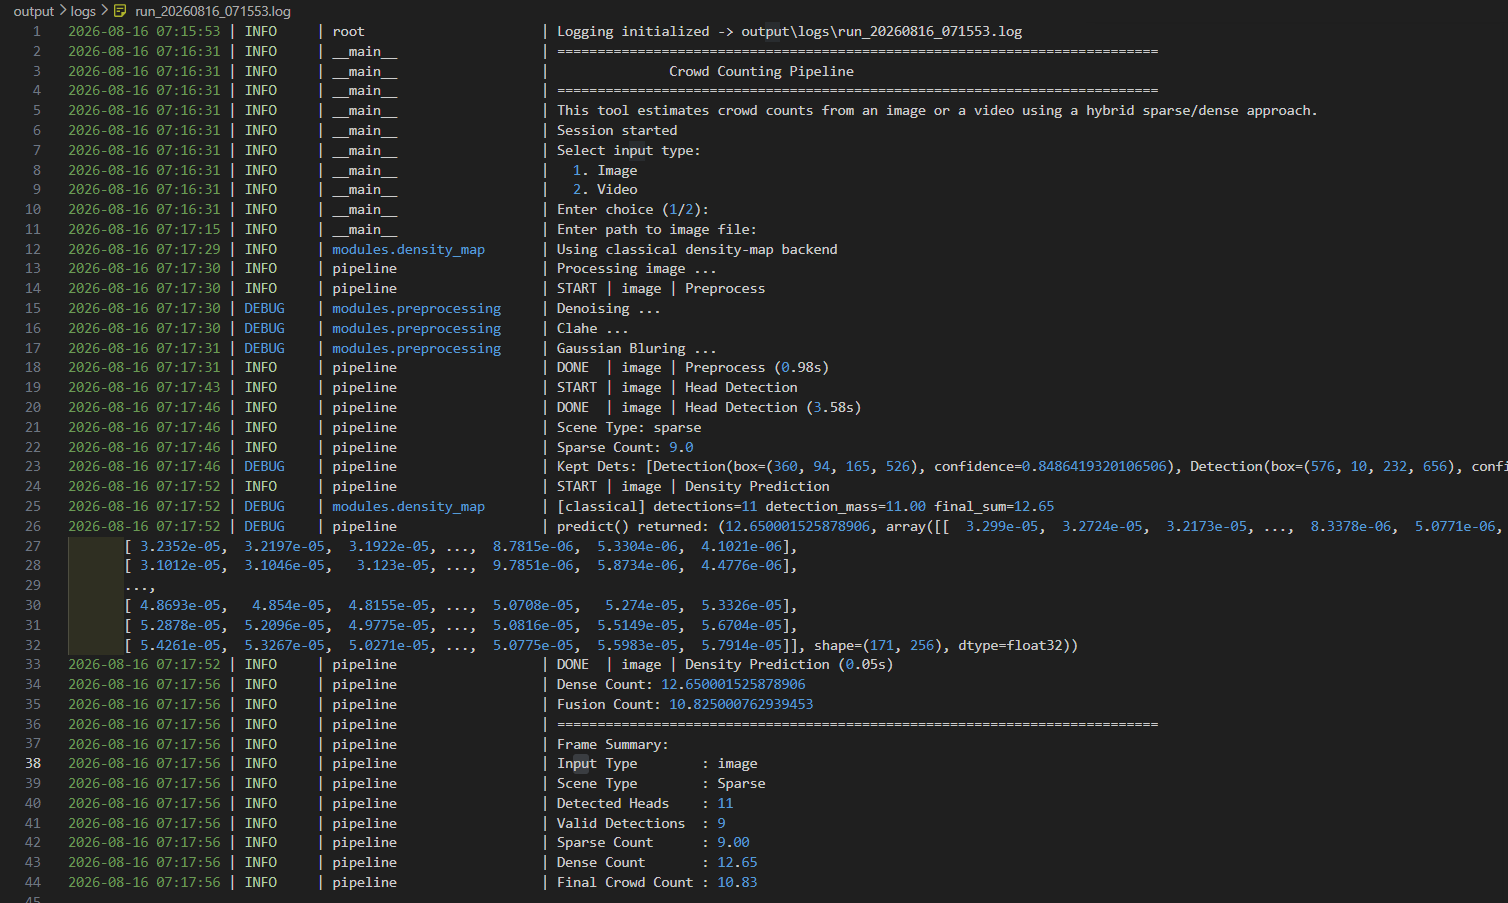
\includegraphics[width=1.00\textwidth]{figures/log_information.png}
    \caption{System execution and processing log information}
    \label{fig:log-information}
\end{figure}

These records support reproducibility, debugging, and post-execution performance analysis. Maintaining separate output artifacts for each processing session also reduces the possibility of unintentionally replacing previously generated results.

Configuration information is maintained separately from runtime generated data. This separation provides a clear distinction between system parameters and generated artifacts, simplifying system maintenance and reducing the possibility of inconsistencies caused by outdated runtime information.

% The file based data management strategy is suitable for the current standalone deployment scenario, particularly for offline analysis of recorded transportation data. However, a more advanced persistence mechanism could be introduced for future deployments involving continuous camera monitoring and large scale occupancy analysis. A database or time series storage system could support efficient storage, querying, historical analysis, and integration with monitoring dashboards.

% ============================================================
\section{Testing and Debugging Approaches}

Testing was conducted using a structured multi level strategy to evaluate the correctness, reliability, and robustness of the proposed passenger counting system. The testing levels and their respective objectives are summarised in Table~\ref{tab:testing-strategy}. The overall testing strategy is illustrated in Figure~\ref{fig:pyramid}.

\begin{figure}[ht]
    \centering
    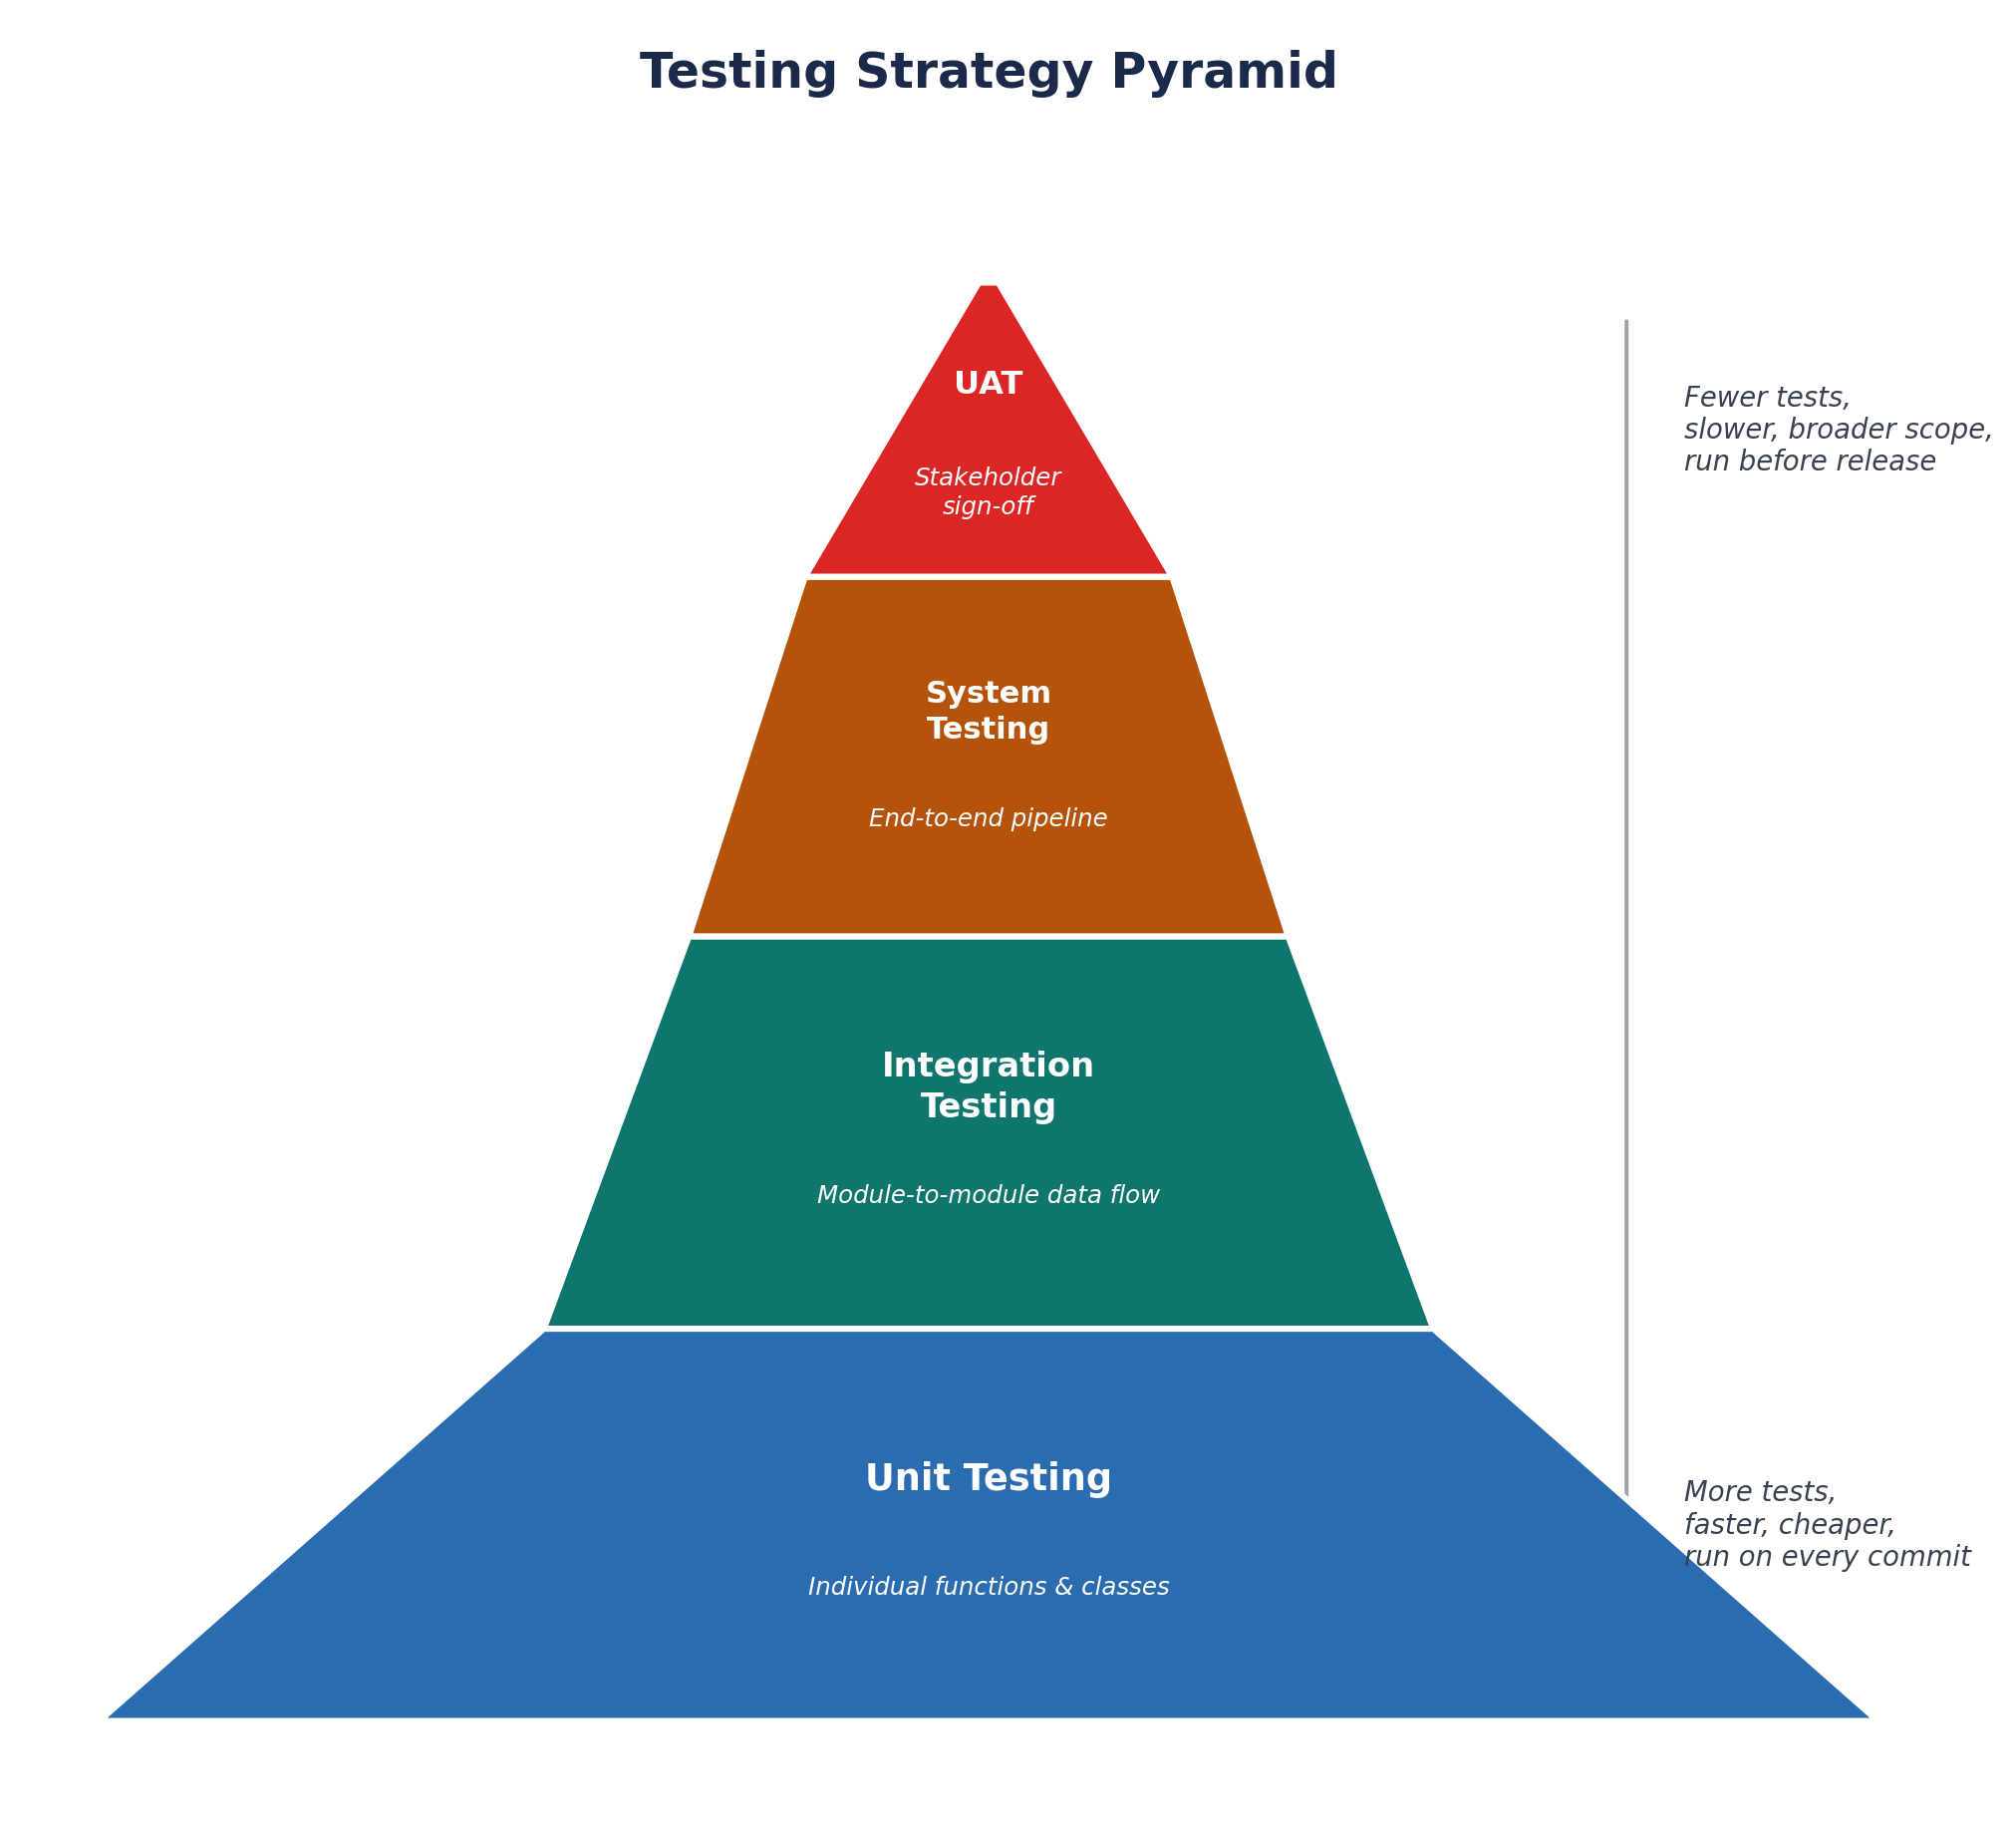
\includegraphics[width=0.62\textwidth]{figures/testing_pyramid.png}
    \caption{Multi-level testing strategy adopted for the proposed system}
    \label{fig:pyramid}
\end{figure}

% ============================================================
% Testing Strategy Table
% ============================================================

\begin{longtable}{|>{\raggedright\arraybackslash}p{3.3cm}|>{\raggedright\arraybackslash}p{4.3cm}|>{\raggedright\arraybackslash}p{6.4cm}|}

\caption{Testing strategy}
\label{tab:testing-strategy} \\

\hline
\textbf{Testing Level} & \textbf{Purpose} & \textbf{Main Focus} \\
\hline
\endfirsthead

\hline
\textbf{Testing Level} & \textbf{Purpose} & \textbf{Main Focus} \\
\hline
\endhead

\hline
\multicolumn{3}{r}{\textit{Continued on next page}} \\
\endfoot

\hline
\endlastfoot

\textbf{Unit Testing}
&
Validate individual components independently.
&
Correctness of preprocessing, detection, density estimation, scene analysis, and fusion operations.
\\
\hline

\textbf{Integration Testing}
&
Verify communication and data exchange between components.
&
Compatibility and correctness of data transferred between consecutive processing stages.
\\
\hline

\textbf{System Testing}
&
Evaluate the complete passenger counting workflow.
&
End-to-end processing of image and video inputs under different crowd density and environmental conditions.
\\
\hline

\textbf{User Acceptance Testing}
&
Evaluate practical usability and output interpretation.
&
Input handling, result presentation, system usability, and suitability for passenger counting analysis.
\\
\hline

\end{longtable}


% ============================================================
\subsection{Debugging Approaches}

Debugging was performed throughout the development and testing process. The primary approaches used to identify and resolve errors are summarised in Table~\ref{tab:debugging-approaches}.

% ============================================================
% Debugging Approaches Table
% ============================================================

\begin{longtable}{|>{\raggedright\arraybackslash}p{3.3cm}|>{\raggedright\arraybackslash}p{4.8cm}|>{\raggedright\arraybackslash}p{5.9cm}|}

\caption{Debugging approaches}
\label{tab:debugging-approaches} \\

\hline
\textbf{Approach} & \textbf{Purpose} & \textbf{Application} \\
\hline
\endfirsthead

\hline
\textbf{Approach} & \textbf{Purpose} & \textbf{Application} \\
\hline
\endhead

\hline
\multicolumn{3}{r}{\textit{Continued on next page}} \\
\endfoot

\hline
\endlastfoot

\textbf{Execution Monitoring}
&
Identify the processing stage responsible for an error.
&
Monitoring processing progress, execution status, and abnormal behaviour.
\\
\hline

\textbf{Stage Isolation}
&
Locate errors within individual processing stages.
&
Testing a specific stage independently when an unexpected result occurs.
\\
\hline

\textbf{Intermediate Result Analysis}
&
Identify errors in numerical and visual outputs.
&
Inspecting density maps, corrected estimates, and filtered detection results.
\\
\hline

\textbf{Visual Inspection}
&
Detect spatial and detection related errors.
&
Examining missed detections, false detections, incorrect locations, and density-estimation patterns.
\\
\hline

\textbf{Input Variation}
&
Identify system behaviour under different conditions.
&
Testing with varying crowd densities, illumination conditions, occlusion levels, and image quality.
\\
\hline

\end{longtable}

The combination of multi level testing and systematic debugging provided a structured approach for identifying errors, validating individual components, and ensuring the reliability of the complete passenger-counting system.

\section{Version Control and Configuration Management}

\subsection{Version Control}

The project uses Git and GitHub for source code version control. Git provides a mechanism for tracking changes, maintaining project history, and managing different versions of the software.

The repository also uses a \texttt{.gitignore} file to prevent unnecessary generated files from being committed. In particular, \texttt{\_\_\allowbreak pycache\_\_} and the \texttt{output/} directory are excluded from version control. This is appropriate because these files are generated during program execution and do not need to be maintained as source code.

\subsection{Configuration Management}

The main configuration management component identified in the repository is
\texttt{requirements\allowbreak.txt}. It contains the project's Python dependencies
with specific versions, allowing the development environment to be reproduced more
consistently.

For example, the project specifies:

\begin{itemize}
    \item NumPy 2.5.1
    \item OpenCV 4.10.0.84
    \item PyTorch 2.13.0
    \item TorchVision 0.28.0
    \item Ultralytics 8.4.99
    \item Matplotlib 3.11.0
\end{itemize}

The requirements file contains 36 pinned dependencies. Pinning package versions is beneficial because different dependency versions can produce different results, particularly in machine-learning and computer vision applications.